\subsection*{Interferenz bei Lichtwellen}
Ziel dieses Versuchs ist die Messung der Wellenlänge eines Lasers und die Bestimmung der Brechzahlen von Luft und $\ce{CO2}$. Ganz zentral ist hierbei die Interferenz von Licht. \\
Für die Erklärung der Interferenz eignet sich die Beschreibung des Lichts als ebene, elektromagnetische Welle
\begin{align}\label{E-Feld}
	\vec{E}(x,t) = \vec{E}_0\cos(kx-\omega t-\delta)
\end{align}
am besten. Man beschränkt sich hier aus Gründen der Einfachheit auf das elektrische Feld und eine Dimension, nämlich die Ausbreitungsrichtung $x$. Die restlichen Größen sind die Wellenzahl $k$, die (Kreis-)Frequenz $\omega$ und ein Phasenverschub $\delta$ bezogen auf einen festen Anfangspunkt. Treffen zwei Lichtwellen aufeinander können sie einfach addiert werden. Das führt bei einem Gangunterschied von $2\pi n$ ($n\in\mathbb{N}$), zwischen den beiden Einzelwellen, zu einer Feldstärke
\begin{align*}
	\vec{E}_{ges}(x,t) &= \vec{E}_{10}\cos(kx-\omega t+2\pi n) + \vec{E}_{20}\cos(kx-\omega t) \\
	&= \left(\vec{E}_{10}+\vec{E}_{20}\right)\cos(kx-wt) \ ,
\end{align*}
bei einem Gangunterschied von $(2n+1)\pi$ dagegen ist die resultierende Gesamtfeldstärke
\begin{align*}
	\vec{E}_{ges}(x,t) &= \vec{E}_{10}\cos(kx-\omega t+(2n+1)\pi) + \vec{E}_{20}\cos(kx-\omega t) \\
	&= \left(\vec{E}_{20}-\vec{E}_{10}\right)\cos(kx-wt) \ .
\end{align*}
Haben die beiden Lichtstrahlen die gleiche Amplitude wird die Feldstärke verdoppelt bzw. komplett ausgelöscht. \\
Da die Feldstärke keine leicht zu messende Größe ist, wird im Versuch die Intensität
\begin{align}
	I = \frac{1}{t_2-t_1}\int_{t_1}^{t_2}\left|\vec{E}(x,t)\right|^2 \text{d}t
\end{align}
verwendet. Der Integrationszeitraum $t_2-t_1$ sollte dabei groß gegenüber der Periodendauer $\frac{2\pi}{\omega}$ sein. Für zwei sich überlagernde elektromagnetische Wellen (hier in komplexer Schreibweise, um die Rechnung zu vereinfachen) aus derselben Quelle (gleiche Amplitude und Frequenz) ist die Intensität dann
\begin{align}
	I &= \frac{\vec{E}_0^2}{t_2-t_1}\int_{t_1}^{t_2}\left|\mathrm{e}^{i(kx-\omega_t-\delta_1)}+\mathrm{e}^{i(kx-\omega t-\delta_2)}\right|^2 \text{d}t \\
	&= \frac{\vec{E}_0^2}{t_2-t_1}\int_{t_1}^{t_2}
	\left(2+2\cos(\delta_2-\delta_1)\right)
	\text{d}t \\
	&\label{Intensitat}= 2\vec{E}_0^2\left(1+\cos(\delta_2-\delta_1)\right) \ .
\end{align}
Demnach kann die Interferenz auch über die Intensität gemessen werden. Sie liegt, abhängig vom Gangunterschied $\delta_2-\delta_1$, zwischen $0$ und $4\vec{E}_0^2$.
\subsection*{Voraussetzungen für die Beobachtung von Interferenz}
Bei alltäglichen Lichtquellen, wie der Sonne oder einer Glühbirne, sind $\delta_1$ und $\delta_2$ keine Konstanten, sondern statistische Funktionen der Zeit, sodass das Integral des Cosinus-Terms über eine lange Zeit $t_2-t_1$ verschwindet und eine konstante Intensität beobachtet wird. Dieses Licht ist nicht interferenzfähig und wird als inkohärent bezeichnet. Kohärentes Licht dagegen kann durch \emph{einen} Ausdruck \eqref{E-Feld} mit festen $k, \omega$ und $\delta$ beschrieben werden. \\
Üblicherweise wird ein Laser verwendet, wenn Licht mit hoher Kohärenz gebraucht wird. Durch einen geeigneten Versuchsaufbau (siehe Abbildung \ref{Gluhlampe}) können allerdings auch bei nichtkohärenten Lichtquellen Interferenz-Erscheinungen beobachtet werden.
\begin{figure}[h!]
	\centering
	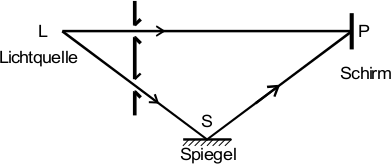
\includegraphics[width=0.6\textwidth]{Koharenz_Gluhlampe.png}
	\caption{Versuchsaufbau, der eine nicht interferenzfähige Lichtquelle für Interferenz-Experimente erlaubt}
	\label{Gluhlampe}
\end{figure} 
Hierbei wird das Licht in zwei kohärente Strahlen geteilt, die so umgelenkt werden, dass sie am Schirm interferieren können. Es gilt zu beachten, dass die Lichtquelle zum Beispiel durch Glühemission Wellenpakete emittiert. Der Emissionsvorgang passiert nicht instantan, sondern dauert eine endliche Zeit $\tau$, woraus eine endliche Länge $l$ des Paketes resultiert. Damit sich die Wellenpakete, nachdem sie unterschiedliche Wege zum Schirm gegangen sind, am Schirm treffen können, darf der Wegunterschied nicht größer als die Kohärenzlänge $l$ sein.